
\chapter{提案手法のその他の工夫}
\label{sec:appendix1}
提案手法によるタグ比較回数をより減らすための工夫として,Last Tag Prediction(LTP) という手法が有効ではないかと考え,シミュレータに実装し評価を行った.本章では,LTP とその評価結果に関して説明する.なお,評価の結果,LTP はあまり効果がないことがわかったため,最終的な提案手法には実装していない.

\section{LTP:Last Tag Prediction}
CONSARVARTIVE 方式 において,第 1 ソース・タグと第 2 ソース・タグがどちらもレディでない命令は,以下のアルゴリズムでセグメントを選択すると述べた.

\begin{itemize}
  \item サブ・セグメントを使用しない場合:第 1 ソース・タグでセグメントを選択する.選択したセグメントに空きがない場合,スワップして第 2 ソース・タグをもとにセグメントを決定する.なおも空きがない場合はストールする.
  \item サブ・セグメントを使用する場合:第 1 ソース・タグでメイン・セグメントを,第 2 ソース・タグでサブ・セグメントを選択する.選択したセグメントに空きがない場合,スワップを行い,第 2 ソース・タグでメイン・セグメントを,第 1 ソース・タグでサブ・セグメントを選択する.スワップしてなおも空きがない場合はストールする.
\end{itemize}

このアルゴリズムにおいて,スワップする場合としない場合に選択されるセグメントのどちらにも空きがある場合を考える.このような場合,CONSERVATIVE のアルゴリズムでは,スワップを行わずにディスパッチするセグメントを決定する.

このような場合に,レディとなるのがより遅く,比較がより多く行われるソース・オペランドのタグ(ラスト・タグ)を第 1 ソース・タグのフィールドに書き込むようにセグメントを選択すれば,タグ比較回数をより多く削減できると考えられる.ただし,ラスト・タグがどちらになるかという情報はデコード時にはわからないため,予測を行う必要がある.

ラスト・タグの予測方法は,論文~\cite{ernst2002}で提案されている.この方法を Last Tag Prediction(LTP)と呼ぶ.以下,LTP による予測とセグメントの選択方法に関して説明する.

\begin{figure}[htb]
  \centering
  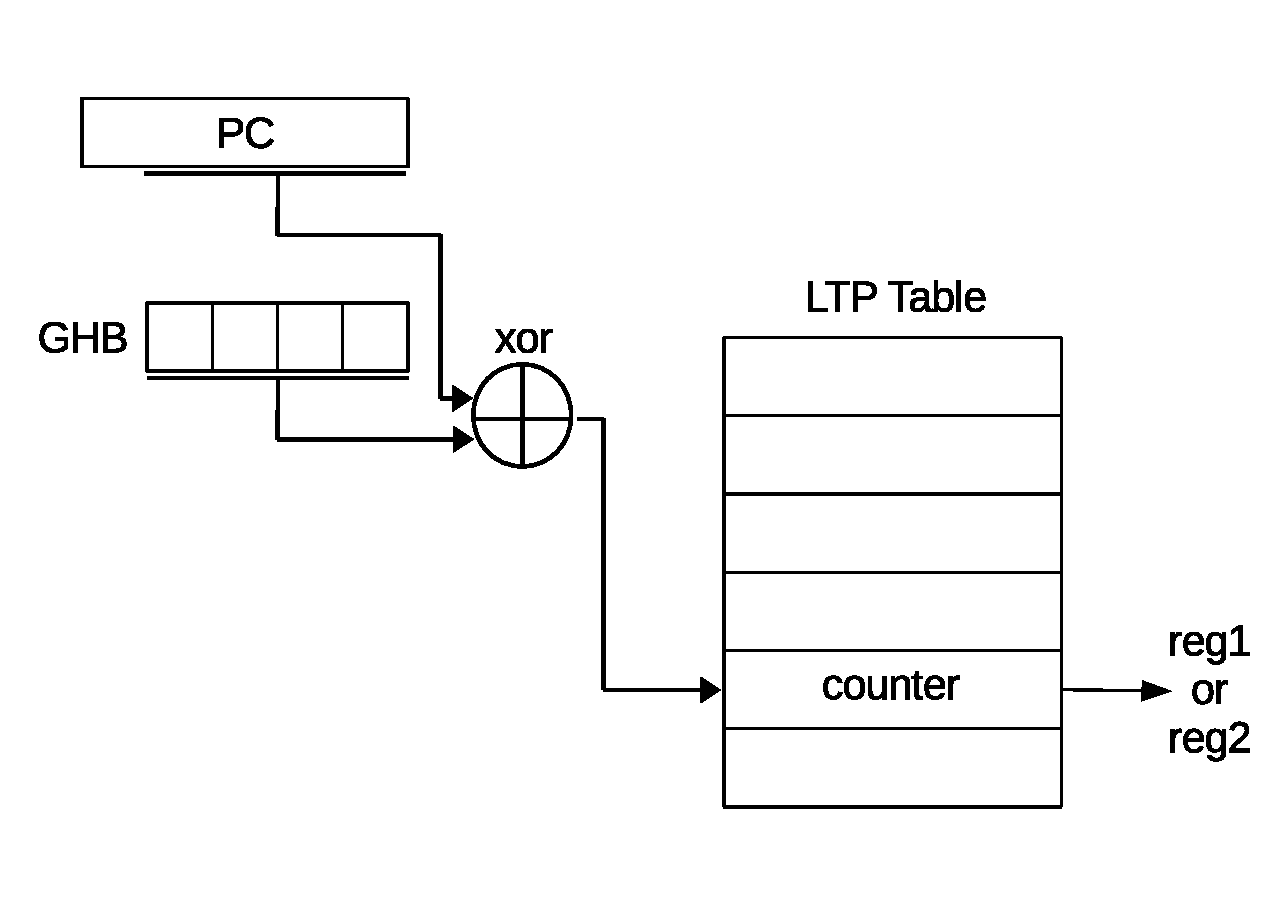
\includegraphics[keepaspectratio, scale=.8]{ltp}
  \caption{LTP の構成}
  \label{fig:ltp}
\end{figure}

LTP は,\fig{ltp}のように.命令の PC の下位ビットビットとグローバル分岐履歴(GHB:Global History Buffer)のハッシュをインデクスとするテーブル(LTP Table)で構成される.LTP Table の各エントリは 2 ビットの飽和型アップ・ダウン・カウンタで構成され,このカウンタは,値が 0 または 1 の場合に第 1 ソース・タグがラスト・タグであることを示し, 2 または 3 の場合に第 2 ソース・タグがラスト・タグであることを示す.予測と学習の方法について説明する.
  
\subsection{予測方法}
命令ディスパッチ時に,第 1 ソース・タグと第 2 ソース・タグがともにレディでなく,なおかつスワップした場合としない場合に選択されるセグメントがいずれもディスパッチ可能な場合に予測が行われる.予測の際には,PC と GHB のハッシュを用いてテーブルを検索し,該当するエントリのカウンタ値を読み出す.

第 1 ソース・タグがラスト・タグであると予測された場合には,スワップを行なわずにセグメントを選択しディスパッチする.第 2 ソース・タグがラスト・タグであると予測された場合には,スワップを行いセグメントを選択し,ディスパッチする.
  

\subsection{学習方法}
学習は命令発行時に,ディスパッチ時に予測を行った命令でのみ行われる.命令発行時に,第 1 ソース・タグと第 2 ソース・タグがレディとなったサイクルを比較する.第 1 ソース・タグ のほうが遅かった場合にはカウンタをデクリメントし,第 2 ソース・タグのほうが遅かった場合にはカウンタをインクリメントする.

\section{LTP の評価}